%------------------------------------------------------------
\chapter{ 磁気流体力学の数値解法}\label{chap:mhd}
%------------------------------------------------------------


%%%%%%%%%%%%%%%%%%%%%%%%%%%%%%%%%%%%%%%%%%%%%%%%%%%%%%%%%%%%%%%%%%%%%%
\section{1次元磁気流体方程式}
%%%%%%%%%%%%%%%%%%%%%%%%%%%%%%%%%%%%%%%%%%%%%%%%%%%%%%%%%%%%%%%%%%%%%%

\begin{equation}
    \frac{\partial \bm{ U}}{\partial t} 
    + \frac{\partial \bm{ F}}{\partial x}=0
\end{equation}
\begin{equation}
    \bm{ U} = \left( 
        \begin{array}{c}
            \rho \\
            \rho v_x \\
            \rho v_y \\
            \rho v_z \\
            E\\
            B_y \\
            B_z \\
    \end{array}
\right),\;\;
    \bm{ F} = \left( 
        \begin{array}{c}
            \rho v_x \\
            \rho v_x^2 + P_T - B_x^2 \\
            \rho v_x v_y  - B_x B_y \\
            \rho v_x v_z  - B_x B_z \\
            (E + P_T)v_x - B_x (\bm{ v}\cdot\bm{ B}) \\
            B_y v_x - B_x v_y\\
            B_z v_x - B_x v_z\\
    \end{array}
\right)
\end{equation}
ここで、$E=P/(\gamma-1) + \rho \bm{ v}^2/2 + \bm{ B}^2/2$は全エネルギー、
$P_T$は全圧力($P+\bm{ B}^2/2$)を表す。
1次元の場合は、$B_x$が一定であれば、$\nabla \cdot \bm{ B}=0$が自動的に
満たされる。

%-----------------------------------------
\clearpage
\subsection{近似Riemann解法}
%-----------------------------------------

%--------------------------------------------------------
\subsubsection{Harten-Lax-van Leer (HLL)近似Riemann解法}
%--------------------------------------------------------

$\bm{ U}_\mathrm{L,R}$
と$\bm{ F}_\mathrm{L,R}$に磁場の効果を含めれば、
流体方程式の場合と全く同じである。

\begin{screen}
\begin{equation}
    \bm{ F}_\mathrm{HLL}
    =\left\{
    \begin{array}{ll}
         \bm{ F}_\mathrm{L} & \mathrm{if~\SL > 0} \\
         \bm{ F}_\mathrm{R} & \mathrm{if~\SR < 0} \\
         \bm{ F}^* & \mathrm{otherwise} \\
    \end{array}
    \right.
\end{equation}
\begin{equation}
\bm{ F}^* = \frac{
\SR \bm{ F}_\mathrm{L}
- \SL \bm{ R}_\mathrm{R}
+ \SR \SL \left(\bm{ U}_\mathrm{R} - \bm{ U}_\mathrm{L}\right)
}{\SR - \SL}
\end{equation}
\end{screen}

\vspace{1cm}

$\SL$と$\SR$は、流体方程式での対応する式の音速をfast波の速度にする。
\begin{equation}
   \SL = \min(v_{x,\mathrm{L}}, v_{x,\mathrm{R}}) -  
    \max(c_\mathrm{f,L}, c_\mathrm{f,R}) ,\;\;\;
   \SR = \max(v_{x,\mathrm{L}}, v_{x,\mathrm{R}}) +  
    \max(c_\mathrm{f,L}, c_\mathrm{f,R}) 
\end{equation}

%--------------------------------------------------------
\clearpage
\subsubsection{HLLC近似Riemann解法}
%--------------------------------------------------------
HLL法と同じように、
$\bm{ U}_\mathrm{L,R}$
と$\bm{ F}_\mathrm{L,R}$に磁場の効果を含めれば、
流体方程式でのHLLC法と基本的には同じである。
接触不連続面の前後で、速度と全圧力($P_\mathrm{T}=P+\bm{ B}^2/2$)が連続であることを使う。

左右に伝播する波の前後での保存則から始める。
\begin{equation}
    \SL \bm{ U}^*_\mathrm{L} - \bm{ F}^*_\mathrm{L}
    = \SL \bm{ U}_\mathrm{L} - \bm{ F}_\mathrm{L}
    \label{hllc_sl}
\end{equation}
\begin{equation}
    \SR \bm{ U}^*_\mathrm{R} - \bm{ F}^*_\mathrm{R}
    = \SR \bm{ U}_\mathrm{R} - \bm{ F}_\mathrm{R}
    \label{hllc_sr}
\end{equation}

\begin{itemize}
\item 質量保存。流体方手式の場合と全く同じ式を得る。
\begin{equation}
 \rho_\mathrm{L}^* (\SL - v_x^*) = \rho_\mathrm{L} (\SL - v_{x,\mathrm{L}}) = C_\mathrm{L},\;\;\;
 \rho_\mathrm{R}^* (\SR - v_x^*) = \rho_\mathrm{R} (\SR - v_{x,\mathrm{R}}) = C_\mathrm{R}
 \label{hllc_mhd_mass}
\end{equation}

\item $x$方向の運動量保存

流体の場合の熱圧力を全圧力に置き換えた式になる。
\begin{equation}
   - P_\mathrm{T}^* + C_\mathrm{L} v_x^* = 
   - P_\mathrm{T,L} + C_\mathrm{L} v_{x,\mathrm{L}},\;\;\;
   - P_\mathrm{T}^* + C_\mathrm{R} v_x^* = 
   - P_\mathrm{T,R} + C_\mathrm{R} v_{x,\mathrm{R}}
 \label{hllc_mhd_momx}
\end{equation}
\begin{screen}
\begin{equation}
    v_x^* = \frac{ - C_\mathrm{L} v_{x,\mathrm{L}} + C_\mathrm{R} v_{x,\mathrm{R}}
    - (P_\mathrm{T,R} - P_\mathrm{T,L})}{-C_\mathrm{L} + C_\mathrm{R}} 
\end{equation}
\begin{equation}
    P_\mathrm{T}^* = P_\mathrm{T,L} + C_\mathrm{L} (v^* - v_\mathrm{L})
        = P_\mathrm{T,R} + C_\mathrm{R} (v^* - v_\mathrm{R})
\end{equation}
\end{screen}
\item $y,z$方向の運動量保存

ここでは$y$方向の方程式のみ示す。$z$方向は、$y$を$z$と置き換えればよい。
\begin{equation}
    C_\mathrm{L} v_{y,\mathrm{L}}^* + B_x B_{y,\mathrm{L}}^* = 
    C_\mathrm{L} v_{y,\mathrm{L}} + B_x B_{y,\mathrm{L}},\;\;\;
    C_\mathrm{R} v_{y,\mathrm{R}}^* + B_x B_{y,\mathrm{R}}^* = 
    C_\mathrm{R} v_{y,\mathrm{R}} + B_x B_{y,\mathrm{R}}  
    \label{hllc_mhd_momy}
\end{equation}

\item $y,z$方向の磁束保存

ここでは$y$方向の方程式のみ示す。$z$方向は、$y$を$z$と置き換えればよい。
\begin{eqnarray}
&&B_x B_{y,\mathrm{L}}^* + (\SL - v_x^*)B_{y,\mathrm{L}}^*
= B_x B_{y,\mathrm{L}} + (\SL - v_{x,\mathrm{L}}) B_{y,\mathrm{L}}\\
&&B_x B_{y,\mathrm{R}}^* + (\SR - v_x^*)B_{y,\mathrm{R}}^*
= B_x B_{y,\mathrm{R}} + (\SR - v_{x,\mathrm{R}}) B_{y,\mathrm{R}}
    \label{hllc_mhd_induc}
\end{eqnarray}
式(\ref{hllc_mhd_momy})と式(\ref{hllc_mhd_induc}を連立させ、
\begin{screen}
\begin{equation}
v_{y,\alpha}^* = v_{y,\alpha}
- B_x B_{y,\alpha} \frac{ v_{x}^* - v_{x,\alpha} } {
C_\alpha (S_\alpha - v_x^*) - B_x^2
}
\end{equation}
\begin{equation}
B_{y,\alpha}^* = B_{y,\alpha}
\frac{ C_\alpha(S_\alpha - v_{x,\alpha}) - B_x^2  } {
C_\alpha (S_\alpha - v_x^*) - B_x^2
}
\end{equation}
\end{screen}
を得る。ここで、$\alpha=(\mathrm{L},\mathrm{R})$となる。
$z$方向の式は
\begin{screen}
\begin{equation}
v_{z,\alpha}^* = v_{z,\alpha}
- B_x B_{z,\alpha} \frac{ v_{x}^* - v_{x,\alpha} } {
C_\alpha (S_\alpha - v_x^*) - B_x^2
}
\end{equation}
\begin{equation}
B_{z,\alpha}^* = B_{z,\alpha}
\frac{ C_\alpha(S_\alpha - v_{x,\alpha}) - B_x^2  } {
C_\alpha (S_\alpha - v_x^*) - B_x^2
}
\end{equation}
\end{screen}
となる。

\item エネルギー保存。

\begin{screen}
\begin{equation}
E_\alpha^* 
= \frac{
(S_\alpha - v_{x,\alpha})E_\alpha - P_{\mathrm{T},\alpha} 
+ P_\mathrm{T}^* v_{x}^* 
+ B_x (\bm{ v}_\alpha \cdot \bm{ B}_\alpha - \bm{ v}_\alpha^* \cdot \bm{ B_\alpha}^*) }
{S_\alpha - v_x^*}
\end{equation}
\end{screen}


\end{itemize}

%--------------------------------------------------------
\clearpage
\subsubsection{HLLD近似Riemann解法}
%--------------------------------------------------------

厳密なMHDリーマン問題では、
片側につき、最も速い伝播速度をもつfast衝撃波、中間的な伝播速度をもつ回転不連続面と、
最も遅い伝播速度のslow衝撃波が伝わる(場合によってはfast希薄波やslow希薄波があり得る)。
左右のslow衝撃波の後面同士が接触不連続面で接している。
HLLC法ではこの中でfast衝撃波のみを考慮に入れていることに対応する。

$B_x$が0でない場合には、垂直方向の運動量保存と誘導方程式から、
接触不連続面の前後で垂直磁場と垂直速度が連続であることが導かれる。
fast衝撃波とslow衝撃波は、その不連続面の前後で磁場の張る平面が回転しないため、初期状態において左右の
磁場の張る平面が異なる場合は、回転不連続面を介して、磁場の張る平面が一致することになる。
HLLD法では、左右に$S_\mathrm{L,R}$で伝播する波の内側に$S_\mathrm{L,R}^*$で伝播する
回転不連続面に対応する波を考慮し、垂直磁場と垂直速度を回転させる。

左右に伝播する回転不連続面の後面の保存量を
$\bm{ U}^{**}_\mathrm{L,R}$とする。
$\SL\Delta t\le x\le \SR\Delta t$において、
$v_x$と全圧力が一定とする。
\begin{equation}
    v^*_{x,\mathrm{L}} = v^{**}_{x,\mathrm{L}}
     = v^{**}_{x,\mathrm{R}}
     = v^{*}_{x,\mathrm{R}} = v^*_x
\end{equation}
\begin{equation}
    P^*_{\mathrm{T,L}} = P^{**}_{\mathrm{T,L}}
     = P^{**}_{\mathrm{T,R}}
     = P^{*}_{\mathrm{T,R}} = P^*_\mathrm{T}
\end{equation}
$S^*_\alpha$前後と、$S_\alpha$の前後の質量保存より
\begin{screen}
\begin{equation}
 \rho^{**}_\alpha = \rho^*_\alpha, \;\;\;
 \rho^*_\alpha  = 
 \rho_\alpha \frac{S_\alpha - v_{x,\alpha}}{S_\alpha - v^*_x} 
 \label{hlld_mhd_mass}
\end{equation}
\end{screen}
を得る。$S_\alpha^*$の前後では$v_x$に差がないので、密度が変化しない。
第2式はHLLC法でのものと同じである。

$S^*_\alpha$前後と、$S_\alpha$の前後の質量保存より
\begin{equation}
 P^{**}_{\mathrm{T},\alpha} = P^*_\mathrm{T}, \;\;\;
 -P^*_\mathrm{T} + C_\mathrm{L} v_x^*  = 
 - P_\mathrm{T,\alpha} + C_\mathrm{L} v_{x,\mathrm{L}}
 \label{hlld_mhd_momx}
\end{equation}
となる。$P_\mathrm{T}$の連続性は、$S^*_\mathrm{T}$を前後での運動量保存
を満たしていることがわかる。式(\ref{hlld_mhd_momx})
の第二式は、HLLCでのものと同じである。
\begin{screen}
\begin{equation}
    v_x^* = \frac{ - C_\mathrm{L} v_{x,\mathrm{L}} + C_\mathrm{R} v_{x,\mathrm{R}}
    - (P_\mathrm{T,R} - P_\mathrm{T,L})}{-C_\mathrm{L} + C_\mathrm{R}} 
\end{equation}
\begin{equation}
    P_\mathrm{T}^* = P_\mathrm{T,L} + C_\mathrm{L} (v^*_x - v_{x,\mathrm{L}})
        = P_\mathrm{T,R} + C_\mathrm{R} (v^*_x - v_{x,\mathrm{R}})
\end{equation}
\end{screen}

$S_\alpha$の前後での$y,z$方向の運動量保存は、HLLCと同じ式を与える。
\begin{screen}
\begin{equation}
v_{y,\alpha}^* = v_{y,\alpha}
- B_x B_{y,\alpha} \frac{ v_{x}^* - v_{x,\alpha} } {
C_\alpha (S_\alpha - v_x^*) - B_x^2
},\;\;\;
v_{z,\alpha}^* = v_{z,\alpha}
- B_x B_{z,\alpha} \frac{ v_{x}^* - v_{x,\alpha} } {
C_\alpha (S_\alpha - v_x^*) - B_x^2
}
\end{equation}
\begin{equation}
B_{y,\alpha}^* = B_{y,\alpha}
\frac{ C_\alpha(S_\alpha - v_{x,\alpha}) - B_x^2  } 
{C_\alpha (S_\alpha - v_x^*) - B_x^2},\;\;\;
B_{z,\alpha}^* = B_{z,\alpha}
\frac{ C_\alpha(S_\alpha - v_{x,\alpha}) - B_x^2  } {
C_\alpha (S_\alpha - v_x^*) - B_x^2
}
\end{equation}
\end{screen}



回転不連続面の伝播速度は流体静止系でAlfv\'en速度
とするのが自然である。
\begin{equation}
    S^*_\mathrm{L} = v^*_x - \frac{|B_x|}{\sqrt{\rho_\mathrm{L}^*}},\;\;\;
    S^*_\mathrm{R} = v^*_x + \frac{|B_x|}{\sqrt{\rho_\mathrm{R}^*}},\;\;\;
    \label{SLRst}
\end{equation}
接触不連続面の前後での保存則を書くと、
\begin{equation}
v^*_x
    \left(
    \begin{array}{c}
       \rho_\alpha^* v^{**}_{y,\mathrm{L}}\\
       \rho_\alpha^* v^{**}_{z,\mathrm{L}} \\
       B^{**}_{y,\mathrm{L}} \\
       B^{**}_{z,\mathrm{L}} 
    \end{array}
    \right)
    - 
    \left(
    \begin{array}{c}
       \rho_\alpha^* v^{**}_{y,\mathrm{L}} v^*_{x} - B_x B^{**}_{y,\mathrm{L}}\\
       \rho_\mathrm{L}^* v^{**}_{z,\mathrm{L}]} v^*_{x} - B_x B^{**}_{z,\mathrm{L}}\\
       B^{**}_{y,\mathrm{L}} v^*_x - B_x v^{**}_{y,\mathrm{L}} \\
       B^{**}_{z,\mathrm{L}} v^*_x - B_x v^{**}_{z,\mathrm{L}} \\
    \end{array}
    \right)
    = v^*_x
    \left(
    \begin{array}{c}
       \rho_\alpha^* v^{**}_{y,\mathrm{R}}\\
       \rho_\alpha^* v^{**}_{z,\mathrm{R}} \\
       B^{**}_{y,\mathrm{R}} \\
       B^{**}_{z,\mathrm{R}} 
    \end{array}
    \right)
    - 
    \left(
    \begin{array}{c}
       \rho_\alpha^* v^{**}_{y,\mathrm{R}} v^*_{x} - B_x B^{**}_{y,\mathrm{R}}\\
       \rho_\mathrm{R}^* v^{**}_{z,\mathrm{R}]} v^*_{x} - B_x B^{**}_{z,\mathrm{R}}\\
       B^{**}_{y,\mathrm{R}} v^*_x - B_x v^{**}_{y,\mathrm{R}} \\
       B^{**}_{z,\mathrm{R}} v^*_x - B_x v^{**}_{z,\mathrm{R}} \\
    \end{array}
    \right)
\end{equation}
となり、直ちに以下の式を得る。
\begin{equation}
    B_x \left(
    \begin{array}{c}
        B^{**}_{y,\mathrm{L}}\\
        B^{**}_{z,\mathrm{L}}\\
        v^{**}_{y,\mathrm{L}} \\
        v^{**}_{z,\mathrm{L}} \\
    \end{array}
    \right)
    = B_x
    \left(
    \begin{array}{c}
        B^{**}_{y,\mathrm{R}}\\
       B^{**}_{z,\mathrm{R}}\\
       v^{**}_{y,\mathrm{R}} \\
      v^{**}_{z,\mathrm{R}} \\
    \end{array}
    \right)
\end{equation}
$B_x\ne 0$のとき、
接触不連続面を介して、垂直磁場と垂直速度が連続となる。
\begin{eqnarray}
  &&  B^{**}_{y,\mathrm{L}} = B^{**}_{y,\mathrm{R}} = B^{**}_y,\;\;\;
   B^{**}_{z,\mathrm{L}} = B^{**}_{z,\mathrm{R}} = B^{**}_z
  \\
  &&  v^{**}_{y,\mathrm{L}} = v^{**}_{y,\mathrm{R}} = v^{**}_y,\;\;\;
    v^{**}_{z,\mathrm{L}} = v^{**}_{z,\mathrm{R}} = v^{**}_z
\end{eqnarray}

次に保存則を使って、$B^{**}_{y,z}$と$v^{**}_{y,z}$を導く。
$S^*_\alpha$の前後での保存則を使うと、
\begin{equation}
S_\mathrm{\alpha}^*
    \left(
    \begin{array}{c}
       \rho_\alpha^* v^{**}_{y,\alpha}\\
       \rho_\alpha^* v^{**}_{z,\alpha} \\
       B^{**}_{y,\alpha} \\
       B^{**}_{z,\alpha} 
    \end{array}
    \right)
    - 
    \left(
    \begin{array}{c}
       \rho_\alpha^* v^{**}_{y,\alpha} v^*_{x} - B_x B^{**}_{y,\alpha}\\
       \rho_\alpha^* v^{**}_{z,\alpha]} v^*_{x} - B_x B^{**}_{z,\alpha}\\
       B^{**}_{y,\alpha} v^*_x - B_x v^{**}_{y,\alpha} \\
       B^{**}_{z,\alpha} v^*_x - B_x v^{**}_{z,\alpha} \\
    \end{array}
    \right)
    = S^*_\alpha
    \left(
    \begin{array}{c}
       \rho_\alpha^* v^{**}_{y,\alpha}\\
       \rho_\alpha^* v^{**}_{z,\alpha} \\
       B^{**}_{y,\alpha} \\
       B^{**}_{z,\alpha} 
    \end{array}
    \right)
    - 
    \left(
    \begin{array}{c}
       \rho_\alpha^* v^{**}_{y,\alpha} v^*_{x} - B_x B^{**}_{y,\alpha}\\
       \rho_\alpha^* v^{**}_{z,\alpha]} v^*_{x} - B_x B^{**}_{z,\alpha}\\
       B^{**}_{y,\alpha} v^*_x - B_x v^{**}_{y,\alpha} \\
       B^{**}_{z,\alpha} v^*_x - B_x v^{**}_{z,\alpha} \\
    \end{array}
    \right)
    \label{jump_SLRst}
\end{equation}
となり、式(\ref{SLRst})を代入すると、
式(\ref{jump_SLRst})の第1式と第3式、そして第2式と第4式が同じ式となり、
$B^{**}_{y,z}$と$v^{**}_{y,z}$の絶対値が決まらない。
これは任意の振幅のAlfv\'en波が許されることで理解される。

次に保存形式の方程式($\partial \bm{ U}/\partial t + 
\partial \bm{ F}/\partial x=0$)
を$\SL\Delta t\le x\le \SR\Delta t$と
$0\le t\le \Delta t$で積分した
\begin{equation}
(\SR-S^*_\mathrm{R})\bm{ U}^*_\mathrm{R}
+ (S^*_\mathrm{R}-v^*_x)\bm{ U}^{**}_\mathrm{R}
+ (v^*_x - S^*_\mathrm{L})\bm{ U}^{**}_\mathrm{L}
+ (S^*_\mathrm{L}- S_\mathrm{L})\bm{ U}^{*}_\mathrm{L}
- \SR \bm{ U}_\mathrm{R}
+  \SL \bm{ U}_\mathrm{L}
+  \bm{ F}_\mathrm{R}
-  \bm{ F}_\mathrm{L}
=0
\end{equation}
を使う。式(\ref{SLRst})より、
\begin{equation}
\left(\SR-v^*_x 
\right)\bm{ U}^*_\mathrm{R}
+ 
\left(\frac{|B_x|}{\sqrt{\rho^*_\mathrm{R}}}\right)
\left( \bm{ U}^{**}_\mathrm{R} - \bm{ U}^*_\mathrm{R}\right)
+ \left(\frac{|B_x|}{\sqrt{\rho^*_\mathrm{L}}}
\right)\left( \bm{ U}^{**}_\mathrm{L}-\bm{ U}^{*}_\mathrm{L}\right)
+ \left(
v^*_x   - S_\mathrm{L}\right)\bm{ U}^{*}_\mathrm{L}
- \SR \bm{ U}_\mathrm{R}
+  \SL \bm{ U}_\mathrm{L}
+  \bm{ F}_\mathrm{R}
-  \bm{ F}_\mathrm{L}
=0
\label{hlld_riemanfan}
\end{equation}
を得る。
$S_\alpha$の前後の保存則
\begin{equation}
 S_\alpha \bm{ U}^*_{\alpha}  - \bm{ F}^*_\alpha
 = S_\alpha \bm{ U}_{\alpha}  - \bm{ F}_\alpha
\end{equation}
を使うと、
\begin{equation}
\left(\frac{|B_x|}{\sqrt{\rho^*_\mathrm{R}}}\right)
\left( \bm{ U}^{**}_\mathrm{R} - \bm{ U}^*_\mathrm{R}\right)
+ \left(\frac{|B_x|}{\sqrt{\rho^*_\mathrm{L}}}
\right)\left( \bm{ U}^{**}_\mathrm{L}-\bm{ U}^{*}_\mathrm{L}\right)
-v^*_x 
\bm{ U}^*_\mathrm{R}
+  v^*_x\bm{ U}^{*}_\mathrm{L}
+  \bm{ F}^*_\mathrm{R}
-  \bm{ F}^*_\mathrm{L}
=0
\label{hlld_riemanfan1}
\end{equation}
を得る。
質量保存と$x$方向の運動量保存については、
$Q^{**}_\alpha=Q^*_\alpha$が満たされる
ので、式(\ref{hlld_riemanfan1})はHLLC法の式と一致する。

$y,z$方向の運動量保存
\begin{equation}
\left(\frac{|B_x|}{\sqrt{\rho^*_\mathrm{R}}}\right)
\left( 
\rho^*_\mathrm{R} v^{**}_{y,z} -
 \rho^*_\mathrm{R} v^{*}_{y,z,\mathrm{R}} 
\right)
+ \left(\frac{|B_x|}{\sqrt{\rho^*_\mathrm{L}}}
\right)\left( 
\rho^*_\mathrm{L} v^{**}_{y,z} -
 \rho^*_\mathrm{L} v^{*}_{y,z,\mathrm{L}} 
\right)
 -B_x B^{*}_{y,z,\mathrm{R}}
 +B_x B^{*}_{y,z,\mathrm{L}}
=0
\label{hlld_riemanfan}
\end{equation}
より、
\begin{screen}
\begin{equation}
 v^{**}_{y,z} =
 \frac{
 \sqrt{\rho^*_\mathrm{L}} v^*_{y,z,\mathrm{L}}
 + \sqrt{\rho^*_\mathrm{R}} v^*_{y,z,\mathrm{R}}
 + \mathrm{sign}(B_x)( B^*_{y,z,\mathrm{R}}- B^*_{y,z,\mathrm{L}})
 }{
  \sqrt{\rho^*_\mathrm{L}} + \sqrt{\rho^*_\mathrm{R}} 
 }
\end{equation}
\end{screen}
$y,z$方向の磁束保存
\begin{equation}
\left(\frac{|B_x|}{\sqrt{\rho^*_\mathrm{R}}}\right)
\left( 
B^{**}_{y,z} -
 B^{*}_{y,z,\mathrm{R}} 
\right)
+ \left(\frac{|B_x|}{\sqrt{\rho^*_\mathrm{L}}}
\right)\left( 
B^{**}_{y,z} -
B^{*}_{y,z,\mathrm{L}} 
\right)
 -B_x v^{*}_{y,z,\mathrm{R}}
 +B_x v^{*}_{y,z,\mathrm{L}}
=0
\label{hlld_riemanfan}
\end{equation}
より、
\begin{screen}
\begin{equation}
 B^{**}_{y,z} =
 \frac{
 \sqrt{\rho^*_\mathrm{R}} B^*_{y,z,\mathrm{L}}
 + \sqrt{\rho^*_\mathrm{L}} B^*_{y,z,\mathrm{R}}
 + \sqrt{\rho^*_\mathrm{R}\rho^*_\mathrm{L}}
 \mathrm{sign}(B_x)( v^*_{y,z,\mathrm{R}}- v^*_{y,z,\mathrm{L}})
 }{
  \sqrt{\rho^*_\mathrm{L}} + \sqrt{\rho^*_\mathrm{R}} 
 }
\end{equation}
\end{screen}

最後に$S^*_\alpha$の前後でのエネルギー保存を使って、$E^{**}_\alpha$を求める。
\begin{equation}
    \left(S^*_\alpha - v^*_x\right)E^{**}_\alpha - 
    P^*_\mathrm{T} v^*_x + B_x (\bm{ v}^{**} \cdot \bm{ B}^{**})
    =  \left(S^*_\alpha - v^*_x\right)E^{*}_\alpha - 
    P^*_\mathrm{T} v^*_x + B_x (\bm{ v}^*_\alpha \cdot \bm{ B}^{*}_\alpha)
\end{equation}
から、
\begin{screen}
\begin{equation}
   E^{**}_\mathrm{L} = E^*_\mathrm{L} - \mathrm{sign}(B_x) 
   \sqrt{\rho^*_\mathrm{L}}
    (   
     \bm{ v}^*_\mathrm{L} \cdot \bm{ B}^{*}_\mathrm{L}
     - 
     \bm{ v}^{**} \cdot \bm{ B}^{**}
    )
\end{equation}
\begin{equation}
   E^{**}_\mathrm{R} = E^*_\mathrm{R} + \mathrm{sign}(B_x) 
   \sqrt{\rho^*_\mathrm{R}}
    (   
     \bm{ v}^*_\mathrm{R} \cdot \bm{ B}^{*}_\mathrm{R}
     - 
     \bm{ v}^{**} \cdot \bm{ B}^{**}
    )
\end{equation}
\end{screen}
を得る。


最終的に、セル境界に当たる状態で場合分けして、以下の数値流束を得る。
\begin{screen}
\begin{equation}
    \bm{ F}_\mathrm{HLLD}
    =\left\{
    \begin{array}{ll}
         \bm{ F}_\mathrm{L} & \mathrm{if~\SL > 0} \\
         \bm{ F}^*_\mathrm{L} =  \bm{ F}_\mathrm{L} + S_\mathrm{L} (\bm{ U}^*_\mathrm{L} -  \bm{ U}_\mathrm{L}) 
         & \mathrm{if}~\SL \le 0 \le S^*_\mathrm{L} \\
         \bm{ F}^{**}_\mathrm{L} = \bm{ F}^*_\mathrm{L} + S^*_\mathrm{L} (\bm{ U}^{**}_\mathrm{L} -  \bm{ U}^*_\mathrm{L}) 
 & \mathrm{if}~S^*_\mathrm{L} \le 0 \le S_\mathrm{M} \\
         \bm{ F}^{**}_\mathrm{R} = \bm{ F}^*_\mathrm{R} + S^*_\mathrm{R} (\bm{ U}^{**}_\mathrm{R} -  \bm{ U}^*_\mathrm{R}) 
 & \mathrm{if}~S_\mathrm{M} \le 0 \le S^*_\mathrm{R} \\
         \bm{ F}^{*}_\mathrm{R} = \bm{ F}_\mathrm{R} + S_\mathrm{R} (\bm{ U}^*_\mathrm{R} -  \bm{ U}_\mathrm{R}) 
 & \mathrm{if}~S^*_\mathrm{R} \le 0 \le S_\mathrm{R} \\
         \bm{ F}_\mathrm{R} & \mathrm{if~}S_\mathrm{R} < 0 \\
    \end{array}
    \right.
\end{equation}
\end{screen}





%%%%%%%%%%%%%%%%%%%%%%%%%%%%%%%%%%%%%%%%%%%%%%%%%%%%%%%%%%%%%%%%%%%%%%
\clearpage
\subsection{実装方針}
%%%%%%%%%%%%%%%%%%%%%%%%%%%%%%%%%%%%%%%%%%%%%%%%%%%%%%%%%%%%%%%%%%%%%%

作成した流体コードを磁気流体コードに書き換えよう。
流体コードでは、基本量($\rho$, $v_x$, $P$)と保存量($\rho$, $\rho v_x$, $E$)の
2つの配列を使って実装した。

磁気流体では横波(Alfv\'en波)が存在するので、
流体では考慮しなかった垂直方向の速度と運動量を新たに加える。
さらに、垂直方向の磁場($B_y$と$B_z$)を加えて、流体変数の数は7個になる。
$\nabla\cdot\bm{B}=0$から$B_x$は一定なので解かなくてよい。

実装方法はいろいろ考えられるが、
今回は表\ref{tab:mhdvar}に示すように、
基本量配列{\ttfamily W}と保存量配列{\ttfamily U}
の両方に$B_y$と$B_z$を加える。
メモリを少し無駄に消費するが、コードが単純になる。
表\ref{sec:mhdvar}は、MHD1次元コードで用いている変数を示している。

\begin{table}[h]
\begin{center}
\caption{1次元磁気流体計算コードにおける流体変数}
\begin{tabular}{|c|c|}
    \hline
    変数名/配列名 & 説明 \\
    \hline
    \hline
    \multicolumn{2}{|l|}{ {\bf 基本量} (primitive variables)} \\
    \hline
    {\ttfamily Q(i,IDN)} & $x=x_i$における密度 (要素数 {\ttfamily nxtot}),   \\
    \hline
    {\ttfamily Q(i,IV1)} & $x=x_i$における$v_x$ (要素数 {\ttfamily nxtot}) \\
    \hline
    {\ttfamily Q(i,IV2)} & $x=x_i$における$v_y$ (要素数 {\ttfamily nxtot}) \\
    \hline
    {\ttfamily Q(i,IV3)} & $x=x_i$における$v_z$ (要素数 {\ttfamily nxtot}) \\
    \hline
    {\ttfamily Q(i,IPR)} & $x=x_i$における圧力 (要素数 {\ttfamily nxtot}) \\
    \hline
    {\ttfamily Q(i,IB2)} & $x=x_i$における$B_y$ (要素数 {\ttfamily nxtot}) \\
    \hline
    {\ttfamily Q(i,IB3)} & $x=x_i$における$B_y$ (要素数 {\ttfamily nxtot}) \\
    \hline
    \multicolumn{2}{|l|}{ {\bf 保存量} (primitive variables) } \\
    \hline
    {\ttfamily U(i,IDN)} & $x=x_i$における密度 (要素数 {\ttfamily nxtot}) \\
    \hline
    {\ttfamily U(i,IM1)} & $x=x_i$における$\rho v_x$ (要素数 {\ttfamily nxtot}) \\
    \hline
    {\ttfamily U(i,IM2)} & $x=x_i$における$\rho v_y$ (要素数 {\ttfamily nxtot}) \\
    \hline
    {\ttfamily U(i,IM3)} & $x=x_i$における$\rho v_z$ (要素数 {\ttfamily nxtot}) \\
    \hline
    {\ttfamily U(i,IEN)} & $x=x_i$における全エネルギー (要素数 {\ttfamily nxtot}) \\
    \hline
    {\ttfamily U(i,IB2)} & $x=x_i$における$B_y$ (要素数 {\ttfamily nxtot}) \\
    \hline
    {\ttfamily U(i,IB3)} & $x=x_i$における$B_z$ (要素数 {\ttfamily nxtot}) \\
    \hline
    \multicolumn{2}{|l|}{ {\bf セル境界の流束} (numerical flux) } \\
    \hline
    {\ttfamily F(i,IDN)} & $x=x_{i+1/2}$における質量流束 (要素数 {\ttfamily nxtot+1}) \\
    \hline
    {\ttfamily F(i,IM1)} & $x=x_{i+1/2}$における運動量流束 (要素数 {\ttfamily nxtot+1}) \\
    \hline
    {\ttfamily F(i,IM2)} & $x=x_{i+1/2}$における運動量流束 (要素数 {\ttfamily nxtot+1}) \\
    \hline
    {\ttfamily F(i,IM3)} & $x=x_{i+1/2}$における運動量流束 (要素数 {\ttfamily nxtot+1}) \\
    \hline
    {\ttfamily F(i,IEN)} & $x=x_{i+1/2}$におけるエネルギー流束 (要素数 {\ttfamily nxtot+1}) \\
    \hline
    {\ttfamily F(i,IB2)} & $x=x_{i+1/2}$における運動量流束 (要素数 {\ttfamily nxtot+1}) \\
    \hline
    {\ttfamily F(i,IB3)} & $x=x_{i+1/2}$における運動量流束 (要素数 {\ttfamily nxtot+1}) \\
    \hline
\end{tabular}
\end{center}
\label{tab:mhdvar}
\end{table}



%%%%%%%%%%%%%%%%%%%%%%%%%%%%%%%%%%%%%%%%%%%%%%%%%%%%%%%%%%%%%%%%%%%%%%
\clearpage
\subsection{高次精度化}
%%%%%%%%%%%%%%%%%%%%%%%%%%%%%%%%%%%%%%%%%%%%%%%%%%%%%%%%%%%%%%%%%%%%%%

%----------------------------
\subsubsection{MUSCL法}
%----------------------------

%Godunov法では、各セル境界$x_{i+1/2}$の左右の状態
%($q_{i+1/2}^\mathrm{L}$, $q_{i+1/2}^\mathrm{R}$)
%を初期値としてRiemann問題を解き、その結果を使って数値流束を求める。
%
%空間一次精度では、格子内の物理量を一様と近似し、
%\begin{eqnarray}
%q_{i+1/2}^\mathrm{L} &=& q_i\\
%q_{i+1/2}^\mathrm{R} &=& q_{i-1}
%\end{eqnarray}
%を用いた。格子内の物理量分布を考えることで、高次精度化できる。
%二次精度では,セル$i$内の$u$の分布を一次関数
%\begin{equation}
%        q(x) = q_i  + \left( \frac{\partial q}{\partial x} \right)_i (x - x_i)
%\end{equation}
%で近似する。
%セル$i$の境界$x_{i+1/2}$での値は,
%\begin{equation}
%        q_{i+1/2}^\mathrm{L} = q_i + \left( \frac{\partial q}{\partial x} \right)_i \frac{ \Delta x}{2}
%\end{equation}
%となり,境界$x_{i-1/2}$での値は,
%\begin{equation}
%        q_{i-1/2}^\mathrm{R} = q_i - \left( \frac{\partial q}{\partial x} \right)_i \frac{ \Delta x}{2}
%\end{equation}
%となる。
%セルでの物理量の勾配は、様々な求め方が考えられるが、例えば、
%\begin{equation}
%        \left( \frac{\partial u}{\partial x} \right)_i = \frac{u_{i+1}- u_{i-1}}{2\Delta x}
%\end{equation}
%で近似する。
%
%
%音波などの解が滑らかな問題であれば、上記の手法で高次精度が得られる。
%しかし(磁気)流体力学では衝撃波など不連続面が頻繁に発生する。
%そのような物理量が急激に変化する場所では
%上記の単純な手法を使うと非物理的な振動が生じることが知られている
%(Godunovの定理)。
%
%一次精度の結果と比較すると形はシャープになるが,非物理的な振動が立ってしまう。
%線形方程式に対しては,
%「二次以上の精度をもつ手法は解の単調性を維持できず,必ず振動する」というGodunovの定理がある
%(例は中心差分)。
%\begin{figure}[htpb]
%        \centering
%        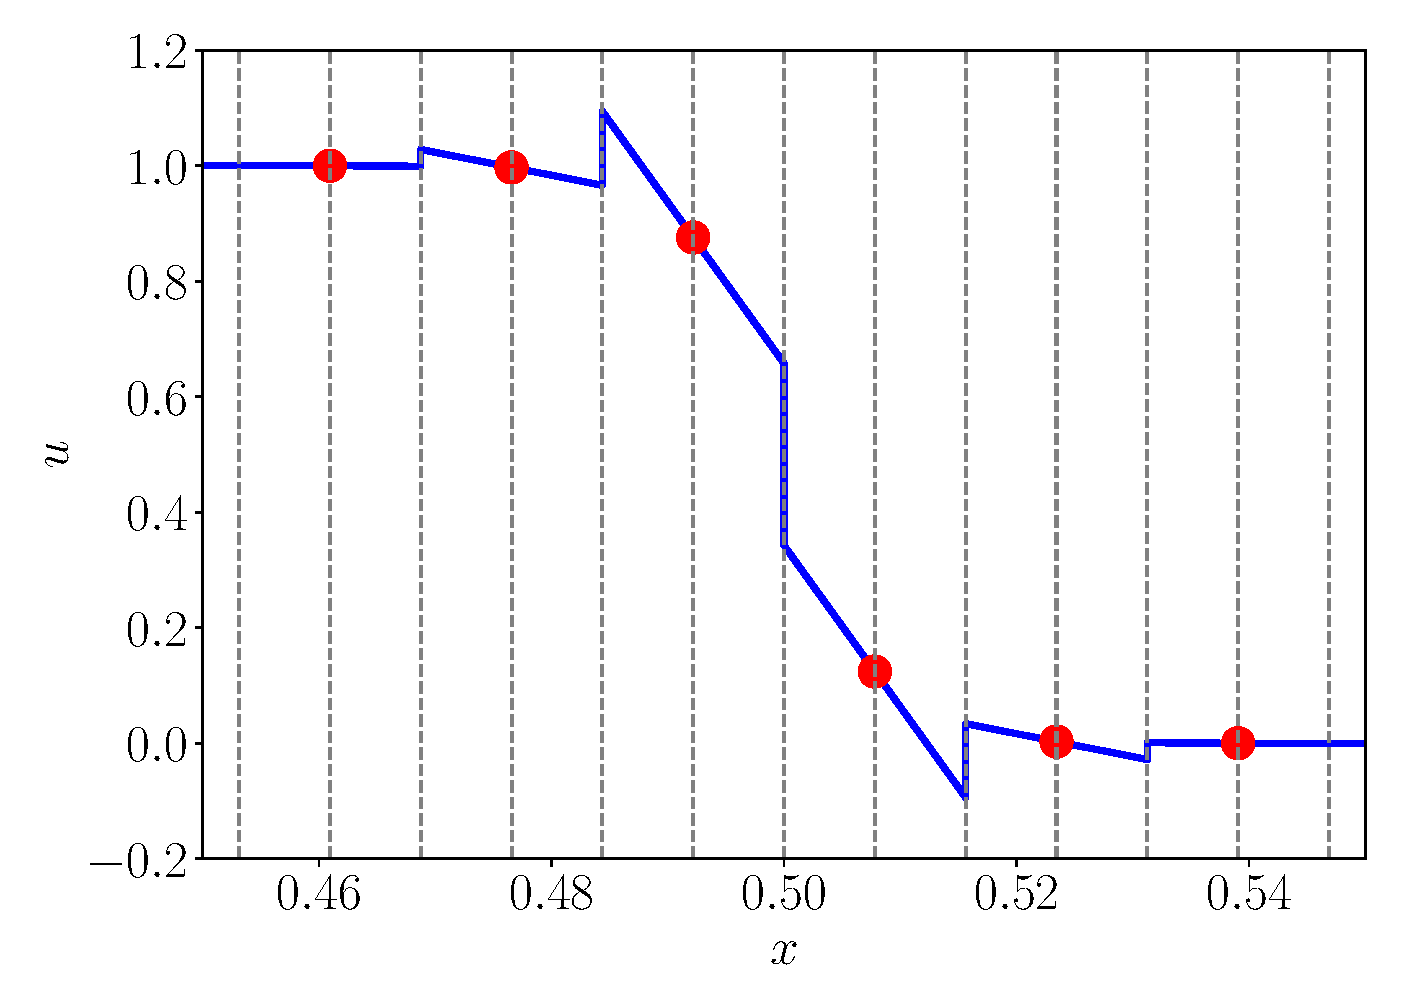
\includegraphics[width=10cm]{2nd.eps}
%        \caption{セル内の$u$の分布を表す。破線はセル境界。}
%        \label{fig:2nd}
%\end{figure}
%図\ref{fig:2nd}は,各セル内の$u$の分布を表す。$u$が急激に変化する場所で,$u_\mathrm{L,R}$が$0\le u\le 1$から
%大きく外れている。このような値を使って流束を求めるために振動が発生する。
%
%
%非物理的な振動を防ぐため,
%現在の宇宙物理学ではMonotonic Upwind Scheme for Conservation Laws(MUSCL)法がよく用いられる。
%MUSCL法ではセル内部の$u$の分布まで含めて,なるべく単調になるように$u$の勾配を制限(limiterと呼ばれる)する。
%多くのlimiterが提案されている。
%
%
%
%代表的なlimiterの一つは,monotonized center(MC)である。
%\begin{equation}
%        \left( \frac{\partial u}{\partial x} \right)_i^{\mathrm{MC}} \Delta x
%        = \left\{
%                \begin{array}{ll}
%                        \mathrm{sgn}\left( \Delta u_{i-1/2} \right)
%                        \min\left( 2|\Delta u_{i-1/2}|, | \Delta u_i |,
%                        2|\Delta u_{i+1/2}|\right)  &  \mathrm{for}\;\;\; \Delta u_{i-1/2} \times \Delta u_{i+1/2}>0 \\
%                        0  &  \mathrm{for}\;\;\; \Delta u_{i-1/2} \times \Delta u_{i+1/2}\le 0 \\
%                \end{array}
%                \right.
%\end{equation}
%ここで$\Delta u_{i+1/2} = u_{i+1} - u_i$,$\Delta u_i = (u_{i+1}-u_{i-1})/2$である。
%単調なところでは,$u_{i+1/2,\mathrm{L}}$と$u_{i-1/2,\mathrm{R}}$が,
%$u_{i+1}$と$u_{i-1}$の間から出ないように制限されている。
%単調ではない極大や極小なところ$\Delta u_{i-1/2}\Delta u_{i+1/2}\le 0$では,勾配が0となる。
%
%MC limiterと近いのはvan Leer limiterである。
%\begin{equation}
%        \left( \frac{\partial u}{\partial x} \right)_i^{\mathrm{vl}} \Delta x
%        = \left\{
%                \begin{array}{ll}
%                        \displaystyle \frac{2\Delta u_{i-1/2}\Delta u_{i+1/2}}{\Delta u_{i-1/2} + \Delta u_{i+1/2}}
%                         &  \mathrm{for}\;\;\; \Delta u_{i-1/2} \times \Delta u_{i+1/2}>0 \\
%                        0  &  \mathrm{for}\;\;\; \Delta u_{i-1/2} \times \Delta u_{i+1/2}\le 0 \\
%                \end{array}
%                \right.
%\end{equation}
%勾配を強く制限するのはminmod limiterである。
%\begin{equation}
%        \left( \frac{\partial u}{\partial x} \right)_i^{\mathrm{minmod}} \Delta x
%        = \left\{
%                \begin{array}{ll}
%                        \mathrm{sgn}\left( \Delta u_{i-1/2} \right)\min\left( |\Delta u_{i-1/2}|,
%                        | \Delta u_{i+1/2}|\right)  &  \mathrm{for}\;\;\; \Delta u_{i-1/2} \times \Delta u_{i+1/2}>0 \\
%                        0  &  \mathrm{for}\;\;\; \Delta u_{i-1/2} \times \Delta u_{i+1/2}\le 0 \\
%                \end{array}
%                \right.
%\end{equation}
%以上のlimiterで制限されたセル内の分布を図\ref{fig:2nd_limiter}に示している。
%$0\le u\le 1$の外に飛び出している部分がなくなっていることがわかる。
%
%その結果,非物理的な振動は消える(図\ref{fig:adv_limiter})。
%minmodは強く勾配を制限するので,空間二次精度であるが,MCやvan-Leer limiterよりも解が拡散的になる。
%
%\begin{figure}[htpb]
%        \centering
%        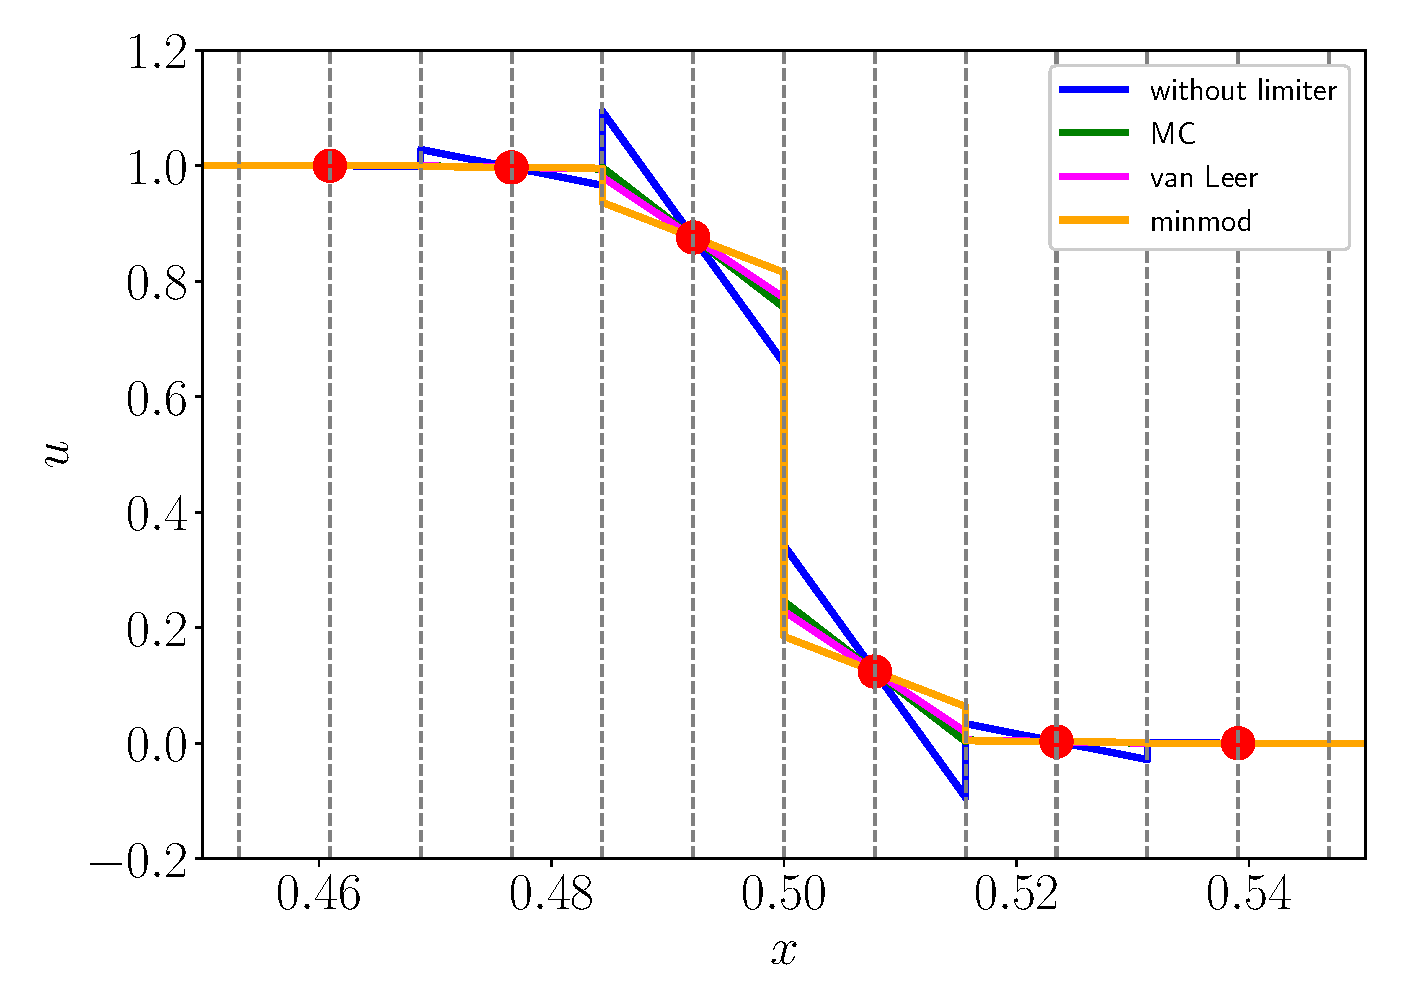
\includegraphics[width=8cm]{2nd_limiter.eps}
%        \caption{セル内の$u$の分布を表す。破線はセル境界。
%                それぞれのlimiterでのセル内の$u$分布を表す。
%        }
%        \label{fig:2nd_limiter}
%\end{figure}
%

%%%%%%%%%%%%%%%%%%%%%%%%%%%%%%%%%%%%%%%%%%%%%%%%%%%%%%%%%%%%%%%%%%%%%%
\clearpage
\section{多次元磁気流体コード}
%%%%%%%%%%%%%%%%%%%%%%%%%%%%%%%%%%%%%%%%%%%%%%%%%%%%%%%%%%%%%%%%%%%%%%

\begin{equation}
    \frac{\partial \bm{ U}}{\partial t} 
    + \frac{\partial \bm{ F}}{\partial x}
    + \frac{\partial \bm{ G}}{\partial y}
    + \frac{\partial \bm{ H}}{\partial z}
    =0
\end{equation}
{\tiny
\begin{equation}
    \bm{ U} = \left( 
        \begin{array}{c}
            \rho \\
            \rho v_x \\
            \rho v_y \\
            \rho v_z \\
            E\\
            B_x \\
            B_y \\
            B_z \\
    \end{array}
\right),\;\;
    \bm{ F} = \left( 
        \begin{array}{c}
            \rho v_x \\
            \rho v_x^2 + P_T - B_x^2 \\
            \rho v_x v_y  - B_x B_y \\
            \rho v_x v_z  - B_x B_z \\
            (E + P_T)v_x - B_x (\bm{ v}\cdot\bm{ B}) \\
            0 \\
            B_y v_x - B_x v_y\\
            B_z v_x - B_x v_z\\
    \end{array}
\right),\;\;
    \bm{G} = \left( 
        \begin{array}{c}
            \rho v_y  \\
            \rho v_y v_x  - B_y B_x \\
            \rho v_y^2 + P_T - B_y^2 \\
            \rho v_y v_z  - B_y B_z \\
            (E + P_T)v_y - B_y (\bm{ v}\cdot\bm{ B}) \\
            B_x v_y - B_y v_x\\
            0 \\
            B_z v_y - B_y v_z\\
    \end{array}
\right),\;\;
    \bm{H} = \left( 
        \begin{array}{c}
            \rho v_z  \\
            \rho v_z v_x  - B_z B_x \\
            \rho v_z v_y  - B_z B_y \\
            \rho v_z^2 + P_T - B_z^2 \\
            (E + P_T)v_z - B_z (\bm{ v}\cdot\bm{ B}) \\
            B_x v_z - B_z v_x\\
            B_y v_z - B_z v_z\\
            0 \\
    \end{array}
\right)
\end{equation}
}









%%%%%%%%%%%%%%%%%%%%%%%%%%%%%%%%%%%%%%%%%%%%%%%%%%%%%%%%%%%%%%%%%%%%%%
\clearpage
\subsubsection{双曲磁場発散除去法}
%%%%%%%%%%%%%%%%%%%%%%%%%%%%%%%%%%%%%%%%%%%%%%%%%%%%%%%%%%%%%%%%%%%%%%



\begin{equation}
    \frac{\partial \bm{ U}}{\partial t} 
    + \frac{\partial \bm{ F}}{\partial x}
    + \frac{\partial \bm{ G}}{\partial y}
    + \frac{\partial \bm{ H}}{\partial z}
    =0
\end{equation}
{\tiny
\begin{equation}
    \bm{ U} = \left( 
        \begin{array}{c}
            \rho \\
            \rho v_x \\
            \rho v_y \\
            \rho v_z \\
            E\\
            B_x \\
            B_y \\
            B_z \\
            \psi \\
    \end{array}
\right),\;\;
    \bm{ F} = \left( 
        \begin{array}{c}
            \rho v_x \\
            \rho v_x^2 + P_T - B_x^2 \\
            \rho v_x v_y  - B_x B_y \\
            \rho v_x v_z  - B_x B_z \\
            (E + P_T)v_x - B_x (\bm{ v}\cdot\bm{ B}) \\
            \psi \\
            B_y v_x - B_x v_y\\
            B_z v_x - B_x v_z\\
            c_h^2 B_x^2 \\
    \end{array}
\right),\;\;
    \bm{G} = \left( 
        \begin{array}{c}
            \rho v_y  \\
            \rho v_y v_x  - B_y B_x \\
            \rho v_y^2 + P_T - B_y^2 \\
            \rho v_y v_z  - B_y B_z \\
            (E + P_T)v_y - B_y (\bm{ v}\cdot\bm{ B}) \\
            B_x v_y - B_y v_x\\
            \psi \\
            B_z v_y - B_y v_z\\
            c_h^2 B_y^2 
    \end{array}
\right),\;\;
    \bm{H} = \left( 
        \begin{array}{c}
            \rho v_z  \\
            \rho v_z v_x  - B_z B_x \\
            \rho v_z v_y  - B_z B_y \\
            \rho v_z^2 + P_T - B_z^2 \\
            (E + P_T)v_z - B_z (\bm{ v}\cdot\bm{ B}) \\
            B_x v_z - B_z v_x\\
            B_y v_z - B_z v_z\\
            \psi \\
            c_h^2 B_z^2
    \end{array}
\right)
\end{equation}
\begin{equation}
    \bm{ U} = \left( 
        \begin{array}{c}
            0\\
            0\\
            0\\
            0\\
            0\\
            0 \\
            0 \\
            0 \\
            \psi/\tau\\
    \end{array}
\right)
\end{equation}
}



\newpage
\subsubsection{Constrained Transport}


%----------------------------------------------------------------------
\clearpage
\section{実習}
%----------------------------------------------------------------------

%-------------------------------------
\subsection{Kelvin-Helmholtz(KH)不安定性}
%-------------------------------------

ファイル群は{\ttfamily multiD/KelvinHelmholtz/}にある。

\subsubsection{理論}
物理状態の異なる流体が接触する不連続面(接触不連続面)
に生じる不安定性の一つである。
$y=0$にある不連続面を介して、$y<0$と$y>0$にそれぞれ一様な
流体1と流体2が存在し、圧力平衡状態にある。
$y<0$と$y>0$にあるガスの物理量を
それぞれ下付き添え字1と2を付けて表す。
流体1と流体2は不連続面に沿った方向に速度$v_{x1}$と$v_{x2}$で
運動している。

微小な揺らぎを与えて、その時間発展を線形解析で
調べる。詳細は参考文献\citep{Chandrasekhar1961}
を読んでもらうことにして、ここでは結果のみを示そう。
非圧縮極限において波数$k$の揺らぎの成長率は、
\begin{equation}
\Gamma = k | v_{x1} - v_{x2} | 
\frac{\sqrt{\rho_1\rho_2}}{\rho_1 + \rho_2}
\end{equation}
で与えられる。成長率は流体間の速度差に比例する。
密度差がある場合は、等密度$\rho_1=\rho_2$のときに
成長率が最大となり、密度差が大きくなるに従い成長率が下がる。
成長率は波数に比例して、小さなスケールの揺らぎが、
より大きな成長率で成長する。これは接触面の厚みが0
と仮定していることが原因である。接触面の厚み$a$を考慮した場合は、
$k>a^{-1}$で成長率が減少する。


次に磁場がある場合について考える。
一様磁場(強度$B$)が接触面に沿っている場合、
成長率は以下のように修正される\citep[例えば][]{Chandrasekhar1961}。
%%%
\begin{equation}
\Gamma = k\sqrt{ ( v_{x1} - v_{x2} )^2 
\frac{{\rho_1\rho_2}}{(\rho_1 + \rho_2)^2} 
- \frac{B^2}{2\pi (\rho_1 + \rho_2)}
}
\end{equation}
%%%
以下の条件を満たすとき、磁場によりKH不安定性が安定化する。
%%%
\begin{equation}
    \frac{ 2B }{
    \sqrt{4\pi \left\{ (\rho_1^{-1} + \rho_2^{-1})/2\right\}^{-1}}}
    > | v_{x1} - v_{x2} | 
\end{equation}
%%%
右辺は
Alfv\'en速度の分母の密度を、
流体1と流体2の密度の調和平均にした形になっている。 
流体1と2で密度が等しい場合、Alfv\'en速度が速度差の半分より
大きいときに安定となる($c_\mathrm{A} > |v_{x1} - v_{x2}|/2$)。

\subsubsection{問題設定と初期条件}

問題設定は各自で自由におこなってもらって構わないが、
ここでは一つの例を挙げる。

計算領域を$-1/2\le x,y\le 1/2$とする。
周期境界条件を使うために、接触面を$y=\pm 1/4$に用意する。
$|y|\le 1/4$の物理量を下付き添え字1を付けて表し、それ以外の領域の物理量を下付き添え字2を
付けて表す。
物理量を滑らかに変化させるため、以下のようにtanhをつかう。
\begin{equation}
\bm{ W}(x,y) = \frac{\bm{ W}_1 - \bm{ W}_2}{2}
\left[ 
\tanh\left( \frac{y+1/4}{h} \right) 
-\tanh\left( \frac{y-1/4}{h} \right) 
\right]
+\bm{ W}_2
\label{kh_ini}
\end{equation}
$h=0.05$は接触面の厚みを表す。

\begin{equation}
\bm{ W}_1 = \left(
\begin{array}{c}
\rho_1 \\
v_{x1} \\
v_{y1} \\
P_1 
\end{array}
\right)
= \left(
\begin{array}{c}
1 \\
v_1 \\
0 \\
1   0
\end{array}
\right),\;\;\;\;
\bm{ W}_2 = \left(
\begin{array}{c}
\rho_2 \\
v_{x2} \\
v_{y2} \\
P_2 
\end{array}
\right)
= \left(
\begin{array}{c}
2 \\
v_2 \\
0\\
10
\end{array}
\right),\;\;\;\;
\end{equation}
流体1の音速は$\sqrt{10\gamma}$で、流体2の音速は$\sqrt{5\gamma}$となる。
非圧縮の線形解析の結果と比較するので、速度差を音速よりも十分小さくする必要がある。
速度差を$v_{x1}-v_{x2} = 1$とする。
したがって、速度差は、流体1にとってはMach数0.24で、流体2にとってはマッハ数0.35である。
速度$v_{x1}$と$v_{x2}$は運動量$\rho_1v_{x1}+\rho_2 v_{x2}$が0になるように入れる。


ここでは接触面を揺らがせるために、
以下の$v_y$を与える。
\begin{equation}
    v_y(x,y) = 10^{-2}\sin(k x) \left\{
    \exp\left[
    - \left( \frac{y+1/4}{w} \right)^2
    \right]
    +\exp\left[
    - \left( \frac{y-1/4}{w} \right)^2
    \right]
    \right\}
\end{equation}
Gauss関数により接触面付近にのみ速度揺らぎが入るようになっている。
$w$はGauss関数の広がりを表し、ここでは例えば$0.1$を採用する。
$x$方向に正弦関数で変動しているため、時間を進めると接触面が波数$k$で揺らぐことになる。


\begin{enumerate}
\item 上記の初期条件と境界条件を設定し、まずは磁場を0としてシミュレーションをおこなう。
可視化をして進化の様子を確認する。

\item 揺らぎの成長率を線形成長率と比較する。様々な方法が考えられるが、
例えば、$y$方向の速度分散の時間進化を調べると簡単。

\item $x$方向に沿った初期磁場を入れる。磁場強度をパラメータとし、成長率の磁場強度依存性を調べ、線形解析の結果と
比較する。
    
\end{enumerate}



%-------------------------------------
\clearpage
\subsection{Rayleigh-Taylor(RT)不安定性}
%-------------------------------------
ファイル群は{\ttfamily multiD/RayleighTaylor/}にある。

\subsubsection{理論}

KH不安定性と同様に、
接触不連続面における不安定性である。
流体1($y<0$)と流体2($y>0$)の間に接触不連続面があり、
$-y$方向に重力(重力加速度の大きさ$g$)が働いている。
成長率は
\begin{equation}
\Gamma^2 = g k \left(
\frac{\rho_2 - \rho_1}{\rho_1 + \rho_2}
\right)
\end{equation}
となり、$\rho_2 > \rho_1$のときに不安定となる。
KH不安定性とは成長率の波数依存性($k$に比例)が弱く、
$\Gamma$は$k^{1/2}$に比例して増加する。


接触面に平行な磁場(強度は$B$)を加えると、成長率が以下のように修正される。
%%%%%%%%%%%%%%%%%%
\begin{equation}
\Gamma^2 = g k \left(
\frac{\rho_2 - \rho_1}{\rho_1 + \rho_2}
- \frac{B^2 k}{2\pi g (\rho_1 + \rho_2)}
\right)
\end{equation}
%%%%%%%%%%%%%%%%%%
KH不安定性とは異なり、$\Gamma=0$を満たす臨界波数$k_\mathrm{cri}$
が定義でき、
$k>k_\mathrm{cri}$を満たす小スケールの揺らぎは磁気張力により
安定化される。

%-------------------------------------
\subsubsection{問題設定と初期条件・境界条件}
%-------------------------------------

RT不安定性をシミュレーションするためには、
運動量保存式とエネルギー方程式に源項が必要である。
今回は重力加速度の大きさを$g$とし$x$負方向に重力をかけると、
\begin{equation}
\left(\frac{\partial \rho v_x}{\partial t}\right)_\mathrm{grav}
= -\rho g
\end{equation}
\begin{equation}
\left(\frac{\partial E}{\partial t}\right)_\mathrm{grav}
= - \rho g v_x
\end{equation}
となる。


計算領域は$-3/4\le x\le 3/4$,$-1/4\le y\le 1/4$とする。
初期条件は、
\begin{equation}
\rho(x,y) = \left\{
\begin{array}{cl}
2 & \mathrm{for}~x\ge 0 \\
1 & \mathrm{for}~x<0
\end{array}
\right.
\end{equation}
\begin{equation}
P(x,y) = P_0 + \rho(x) g x
\end{equation}
\begin{equation}
v_x(x,y) = A \{1+\cos(2\pi x/L_x) \}\{-\cos(2\pi y/L_y)\} ,\;\;v_y(x,y) = v_z(x,y) = 0
\end{equation}
\begin{equation}
    B_x(x,y) = 0,\;\;B_y(x,y) = B_0,\;\;B_z(x,y)=0
\end{equation}
とする。
重力加速度の大きさは$g=0.1$とし、$P_0=2.5$とする。
$y$方向に一様な初期磁場を置く。
摂動は初期不連続面を波数$2\pi/L_y$の波で揺らがせるように,$v_x$に入れる。$A$は初期摂動の大きさを表す。


$y$方向は周期境界条件を課す。
$x$方向の境界条件は、揺らぎが0の場合に平衡状態$\partial P/\partial x=\rho g$を維持できるように設定する。
例えば以下の境界条件を設定する。
\begin{itemize}
    \item  $\rho$と$v_y$、$v_z$、$\bm{B}$, $\phi$は勾配0境界にする。
    \item  $v_x$に対しては反射境界を課す。
    \item  $P$については、与えられた密度分布における平衡分布
    $\partial P/\partial x=\rho g$を数値積分して代入する。
\end{itemize}


%-------------------------------------
\newpage
\subsubsection{課題}
%-------------------------------------
\begin{enumerate}
\item 上記の初期条件と境界条件を設定し、まずは磁場を0としてシミュレーションをおこなう。
可視化をして進化の様子を確認する。{\ttfamily MakeAnime.py}

\item 揺らぎの成長率を線形成長率と比較する。例えば、$x$方向の速度分散の時間進化を調べると簡単。

\item $y$方向に沿った初期磁場を入れる。磁場強度をパラメータとし、成長率の磁場強度依存性を調べ、線形解析の結果と
比較する。
    
\end{enumerate}

\begin{figure}[htpb]
    \centering
    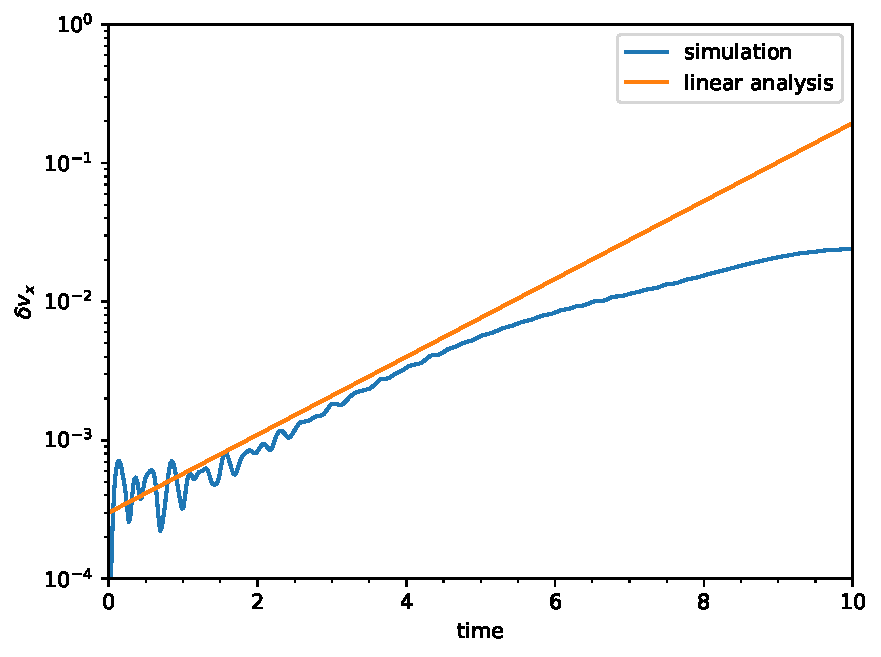
\includegraphics[width=10cm]{figs_mhd/vx_evo.pdf}
    \caption{成長率との比較($B_0=0$)}
    \label{fig:my_label}
\end{figure}

\begin{figure}[htpb]
    \centering
    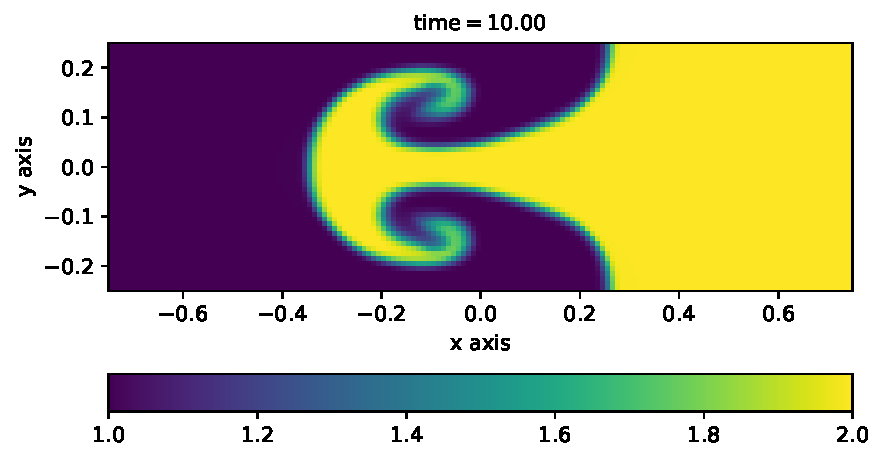
\includegraphics[width=10cm]{figs_mhd/snap00010.pdf}
    \caption{$t=10$における密度分布($B_0=0$)}
    \label{fig:my_label}
\end{figure}



%-------------------------------------
\clearpage
\subsection{Decaying Turbulence}
%-------------------------------------

ファイル群は{\ttfamily multiD/DecayingTurbulence/}にある。


